%!TEX root = ../../main.tex

\chapter{Theoretische Grundlagen}

\section{Unwucht}
Eine Unwucht ist eine Rotation eines rotierenden Körpers, welche leicht versetzt zur Hauptträgheitsachse stattfindet.
Unwuchten erzeugen drehzahlabhängigen Vibrationen, welche zu einem erhöhten Verschleiß, bis hin zu der Zerstörung des gesamten Systems führen können.
Diese enstehen bei einem Rotationskörper, wenn sich der Schwerpunkt nicht auf der Rotationsachse befindet und damit die Fliehkräfte nicht mehr gegenseitig aufgehoben werden können. \cite{unwucht_wiki:2011}

Es wird zwischen zwei Arten von Unwuchten unterschieden:
\begin{itemize}
    \item Statische Unwucht
    \item Dynamische Unwucht
\end{itemize}

Statische Unwucht entsteht, wenn an einem vollkommen ausgewuchteten Rotationskörper auf der Radialebene eine Schwerpunktverlagerung stattfindet. Beispielhaft ist dies in Abbildung \ref{fig:static_imbalance} dargestellt.
Dadurch entstehen kreisförmige Schwingungen rechtwinklig zur Rotationsachse.
\begin{figure}[H]
    \centering
    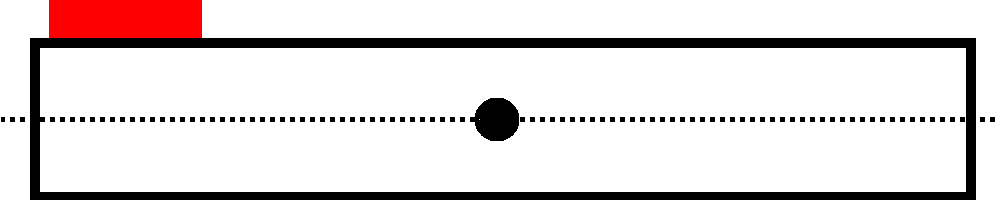
\includegraphics[width=8cm]{images/chapter/02/static_imbalance.png}
    \caption{Bildliche Darstellung einer statischen Unwucht}
    \label{fig:static_imbalance}
\end{figure}

Die dynamische Unwucht tritt auf, wenn sich zwei gleich große, aber zueinander entgegengesetzt liegende Unwuchten in unterschiedlichen Radialebenen befinden, wie in Abbildung \ref{fig:dynamic_imbalance} abgebildet.
Hierdurch fängt die Rotationsachse an sich hin- und herzubewegen, während der Schwerpunkt des Rotationskörpers in Ruhelage verbleibt.
Diese Art der Unwucht macht sich jedoch erst bei sehr hohen Drehzahlen bemerkbar \cite[S. 8]{vibromatrix:2007}.
\begin{figure}[H]
    \centering
    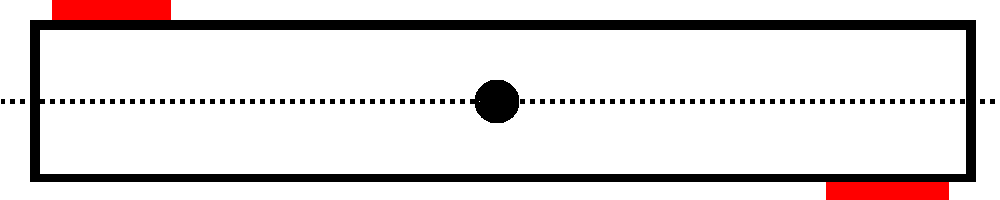
\includegraphics[width=8cm]{images/chapter/02/dynamic_imbalance.png}
    \caption{Bildliche Darstellung einer dynamischen Unwucht}
    \label{fig:dynamic_imbalance}
\end{figure}

\section{Mikrocontrollerplattform Arduino}
\textit{Arduino} ist eine aus Soft- und Hardware bestehende Plattform, dessen Komponenten nach dem Prinzip von OpenSource durch die Lizenzen \ac{LGPL} oder \ac{GPL} komplett quelloffen gehalten werden.
Die Hardware besteht aus einem E/A-Board mit aufgebrachtem Mikrocontroller und mehreren digitalen, als auch analogen Ein- und Ausgängen.
Beispielhaft ist dies in Abbildung \ref{fig:arduino_uno_schema} anhand eines Arduino UNOs dargestellt.
\begin{figure}[H]
	\centering
	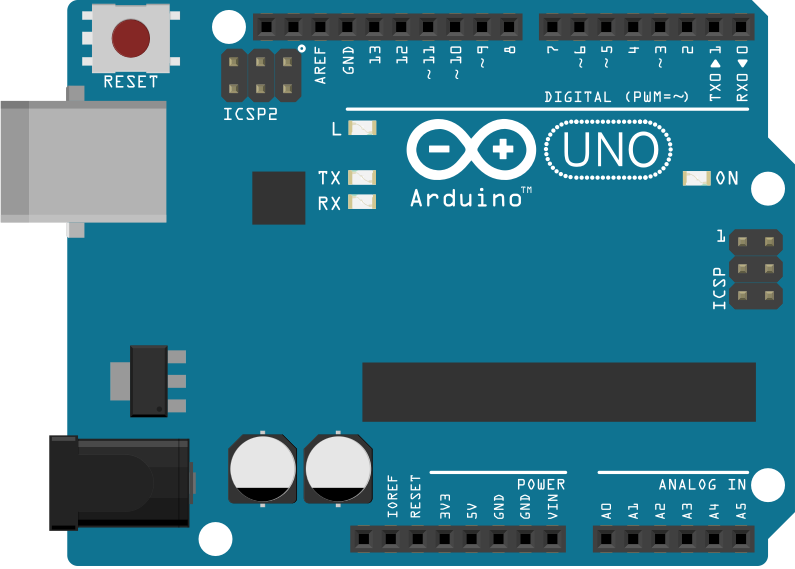
\includegraphics[width=8cm]{images/chapter/02/arduino_uno.png}
	\caption{Schamtische Darstellung eines Arduino UNOs}
	\label{fig:arduino_uno_schema}
\end{figure}
Die Boards stellen eine serielle Schnittstelle, unter anderem auch \ac{USB} zur Verfügung, über welche unter anderem die Programmierung des Mikrocontrollers stattfindet.
Die Software für den Arduino wird in einer C, bzw. C++ ähnlichen Programmiersprache geschrieben.
Das Code-Beispiel in Listing \ref{lst:arduino} stellt ein Programm für ein Blicklicht dar und zeigt die verwendete Sprache beispielhaft.
In dem Listing \ref{lst:arduino} ist ein Code-Beispiel abgebildet, welche diese zeigt.
Für das Entwickeln des Programmes und das Programmiern des Mikrocontrollers wird von dem Hersteller eine Entwicklungsumgebung zur Verfügung gestellt, welche diese Aufgaben vereinfacht.

\begin{lstlisting}[language=C, label={lst:arduino}, caption=Beispiel-Code eines Blinklichtes für den Arduino]
int ledPin = 13;

void setup() {
    pinMode(ledPin, OUTPUT);
}

void loop() {
    digitalWrite(ledPin, HIGH);
    delay(1000);
    digitalWrite(ledPin, LOW);
    delay(1000);
}
\end{lstlisting}

Ein erfolgreiches Konzept der Arduino-Plattform sind die sogenannten \textit{Shields}.
Diese sind Zusatzleiterplatinen welche unkompliziert auf das Arduino-Board gesteckt werden und so die Funktionsvielfalt des Arduinos erweitern.
Ein besonderes Merkmal hierbei ist die Möglichkeit, dass mehrere \textit{Shields} aufeinander gesteckt werden können um so platzsparend mehrere Zusatzleiterplatinen an ein einzelnes Arduino-Board anzuschließen.
\begin{figure}[H]
	\centering
	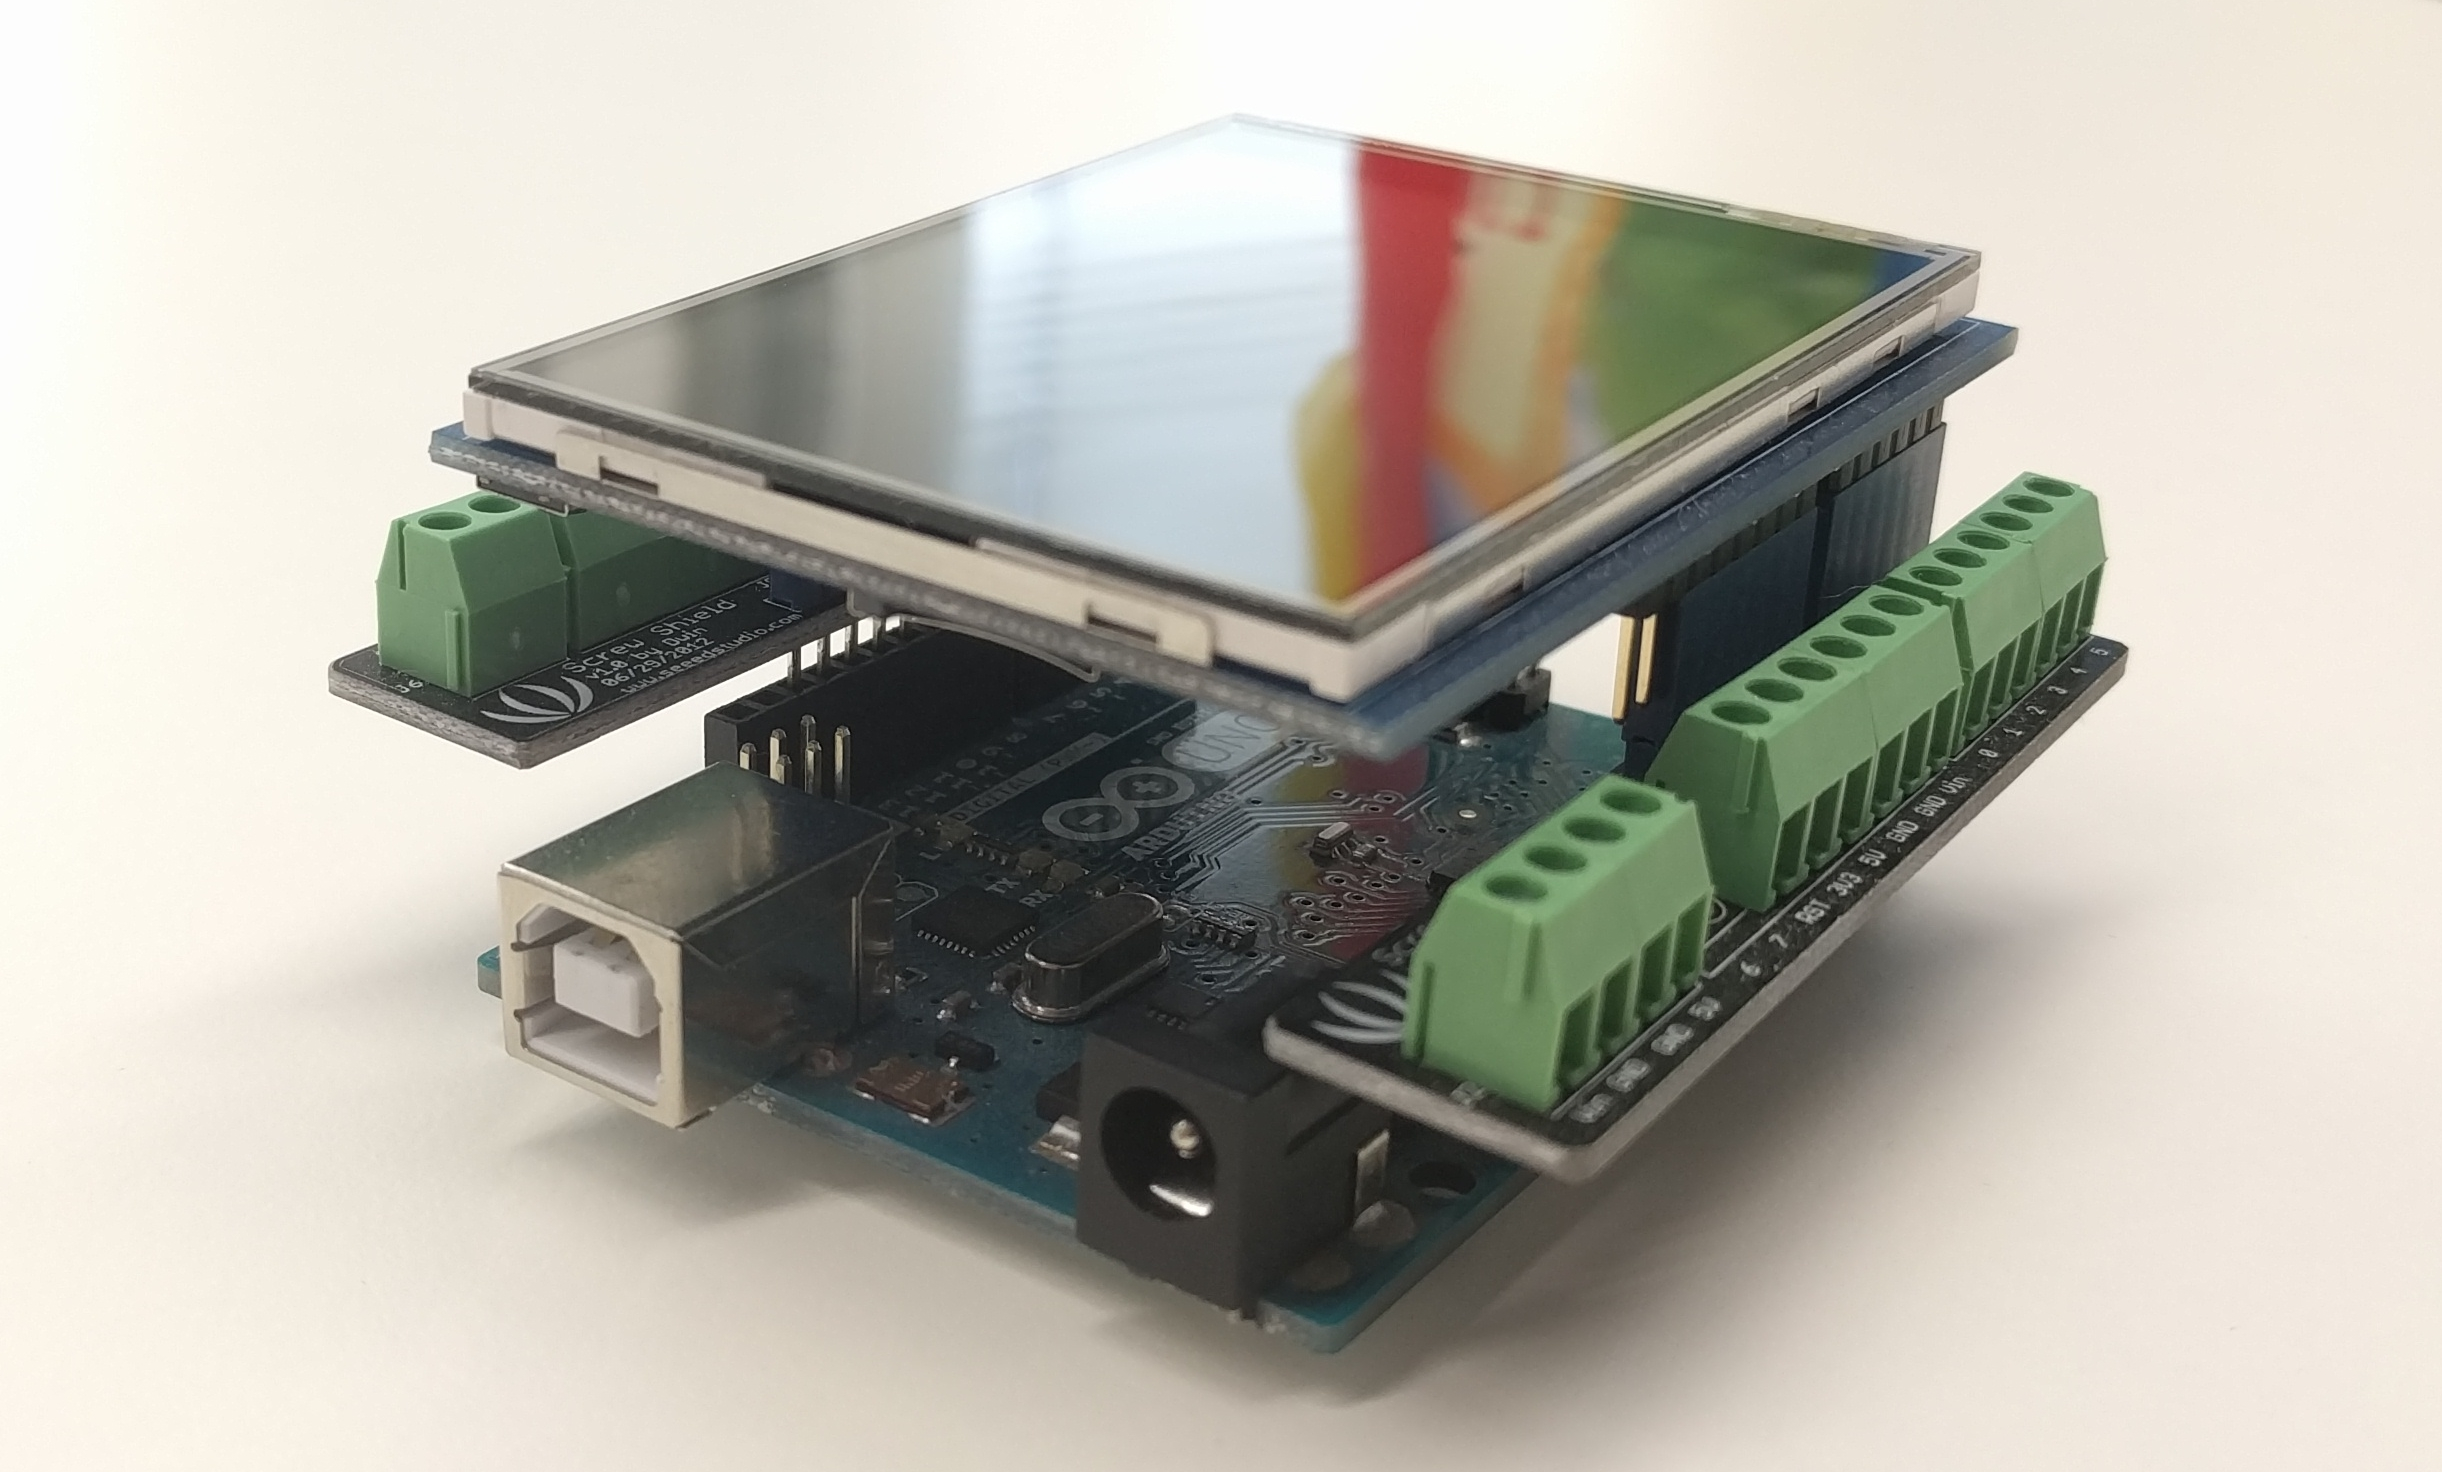
\includegraphics[width=12cm]{images/chapter/02/arduino_shields.jpg}
	\caption{Photografie eines Arduino UNOs mit zwei Shields}
	\label{fig:arduino_shield}
\end{figure}
